\section{The condition $\curl \mbf{u}_h\cdot\mbf{n}=0$ on $\Gamma$}
Let $\Omega\subset\R^3$ be a bounded simply-connected domain with a
Lipschitz continuous boundary $\Gamma$. Let $\Gamma_0,\dots,\Gamma_I$
be the connected components of $\Gamma$.\\

We will use the following notations :
\begin{align*}
gradient(v)&=(\partial_x v, \partial_y v, \partial_z v)=\grad v\\
gradient(\mbf{v})&=\begin{pmatrix}
\partial_x v_x & \partial_y v_x & \partial_z v_x\\
\partial_x v_y & \partial_y v_y & \partial_z v_y\\
\partial_x v_z & \partial_y v_z & \partial_z v_z
\end{pmatrix}=\grad\mbf{v}\\
divergence(\mbf{v})&=\frac{\partial v_x}{\partial x}+\frac{\partial v_y}{\partial y}+\frac{\partial v_z}{\partial z}=\div \mbf{v}\\
rotationnel(\mbf{v})&=\begin{pmatrix}
\partial_y v_z - \partial_z v_y\\
\partial_z v_x - \partial_x v_z\\
\partial_x v_y - \partial_y v_x
\end{pmatrix}=\curl \mbf{v}\\
bcurl(curl(\mbf{v}))&=\curll \mbf{v}\\
H^1(\Omega) &= \{v \in L^2(\Omega)\;|\; \grad v\in L^2(\Omega)\}\\
H^1_0(\Omega) &= \{v \in H^1(\Omega)\; |\; v\restr{\Gamma} = 0\}\\
H(\mathrm{div};\Omega) &= \{\mbf{v} \in [L^2(\Omega)]^3\; |\; \div\mbf{v} \in L^2(\Omega) \}\\
H(\mathrm{curl};\Omega) &= \{\mbf{v} \in [L^2(\Omega)]^3\; |\; \curl\mbf{v} \in L^2(\Omega) \}\\
L^2_\sigma(\Omega) &= \{\mbf{v} \in [L^2(\Omega)]^3\; |\; \div \mbf{v} = 0\text{ et }\mbf{v}\cdot \mbf{n}\restr{\Gamma} = 0 \}\\
D^1(\Omega) &= \{\mbf{v} \in [H^1(\Omega)]^3\cap L^2_\sigma(\Omega)\; |\; (\curl \mbf{v}\cdot \mbf{n})\restr{\Gamma} = 0  \}
\end{align*}

\subsection{Problem}
We consider the following problem :
\begin{pb}\label{pbstart}
Find $\lambda\in\CC$ and $\mbf{u}\ne 0$ such that
\begin{empheq}[left=\empheqlbrace]{align}
\curl\mbf{u} = \lambda\mbf{u} & \quad \mbox{in }\Omega \label{pbstart1}\\
\div\mbf{u} = 0 & \quad \mbox{in }\Omega \label{pbstart2}\\
\mbf{u}\cdot \mbf{n} = 0 & \quad \mbox{on }\Gamma \label{pbstart3}
\end{empheq}
\end{pb}

According to R. Rodriguez and P. Venegas in \cite{Venegas2013}, this problem,
for $\lambda\ne 0$, is equivalent to :
\begin{pb}\label{pbcond}
Find $\lambda\in\CC$ and $\mbf{u}\in
  H(\mathrm{curl};\Omega),\mbf{u}\ne 0$ such that
\begin{empheq}[left=\empheqlbrace]{align}
\curl \mbf{u} = \lambda \mbf{u} & \quad \mbox{in }\Omega \label{pbcond1}\\
\curl \mbf{u}\cdot\mbf{n} = 0 & \quad \mbox{on }\Gamma \label{pbcond2}
\end{empheq}
\end{pb}
Indeed, we have that $(\ref{pbcond1})\implies(\ref{pbstart2})$ since
$\div\mbf{u}=\lambda\div(\curl\mbf{u})=0$. And $(\ref{pbcond1})-(\ref{pbcond2})
\implies (\ref{pbstart3})$ since $\mbf{u}\cdot\mbf{n} =
\lambda\curl\mbf{u}\cdot\mbf{n} = 0$. In the same way,
$(\ref{pbstart1})-(\ref{pbstart3})\implies (\ref{pbcond2})$.\\

The solution of this problem belongs to $\ZZ=\{\mbf{v}\in
H(\mathrm{curl};\Omega \,|\, \curl\mbf{v}\cdot\mbf{n}=0 \mbox{
  on } \Gamma \}$.\\
This space already appeared in \cite{girault90-1} and we know that each functions $\mbf{v}\in\ZZ$ has the decomposition
\begin{equation}\label{relation} \mbf{v}=\mbf{w} + \grad q \end{equation}
with $q\in H^1(\Omega)$ and $\mbf{w}\in [H^1(\Omega)]^3$ with div $\mbf{w} = 0$ on $\Omega$ and $\mbf{w}\times\mbf{n} = 0$ on $\Gamma$. All the functions of this form belong to $\ZZ$.\\

Next, we multiply by $\mbf{v}\in\ZZ$ and integrate :
\[ \int_\Omega \curl\mbf{u}\cdot\mbf{v} = \lambda\int_\Omega
\mbf{u}\cdot\mbf{v} \]
We have the follwing property for all $\mbf{x},\mbf{y}\in\ZZ$ :
\[ \int_\Omega \left(\curl\mbf{x}\right)\cdot\mbf{y} -
\mbf{x}\cdot\left(\curl\mbf{y}\right) = 0 \]
Then, by applying it and using
$\mbf{u}=\curl\mbf{u}/\lambda$, we obtain the following
variationnal form of the Problem \ref{pbstart} :
\begin{pb}\label{pbweak}
Find $\lambda\in\CC$ and $\mbf{u}\in\ZZ$, $\mbf{u}\ne 0$, such
that
\[ \int_\Omega \curl\mbf{u}\cdot\curl\mbf{v} =
\lambda^2\int_\Omega \mbf{u}\cdot\mbf{v} \quad \forall
\mbf{v}\in\ZZ \]
\end{pb}

If $(\lambda,\mbf{u})$ is a solution of Problem \ref{pbstart}, then it is a
solution of Problem \ref{pbweak}. But the contrary is not always true,
see \cite{Venegas2013} Corollary 3.10 :\\

If $\nu\ne 0$ is a solution of Problem \ref{pbweak} and $\bm{\mathcal{E}}$ the
corresponding eigenspace, then there exists an eigenvalue $\lambda$ of
Problem \ref{pbstart} such that $\nu=\lambda^2$ and $\bm{\mathcal{E}}$ is an
invariant subspace of Problem \ref{pbstart}.\\

In fact, the eigenfunctions of Problem \ref{pbweak} are not necessarily
eigenfunctions of Problem \ref{pbstart}. If both $\lambda$ and $-\lambda$
are eigenvalues of Problem \ref{pbstart}, the $\lambda^2$ is an eigenvalue
of Problem \ref{pbweak} with multiplicity equal to the sum of those of
$\lambda$ and $-\lambda$. And the eigenfunction of Problem \ref{pbweak}
corresponding to $\lambda^2$ would be a linear combination of the
eigenfunctions of Problem \ref{pbstart} associated to $\lambda$ and
$-\lambda$.\\

\begin{rk}
In our case, we are mainly interested by the eigenspace, since the
eigen functions span the space $D^1(\Omega)$. We use the fact that
$\curl\mbf{u}=\lambda\mbf{u}$ but it is a convenience, we could
also compute $\curl\mbf{u}$.
\end{rk}

\subsection{Discretization}
From now on, we'll use the following notations :
\begin{align*}
&\TT_h\mbox{ the set of tetrahedra } T \mbox{ such that }
\mbox{ such that } \Omega=\cup_{T\in\TT}T\\
&\TT_h^\Gamma =\{F\mbox{ faces of } T\in \TT_h \,|\, F\subset \Gamma
\}\\
&\NN^k(T)=[\PP_{k-1}(T)]^3\oplus\{\mbf{p}\in[\PP_k(T)]^3 \,|\,
\mbf{p(x)}\cdot\mbf{x}=0 \}\\
&\NN_h=\{\mbf{v}_h\in H(\mathrm{curl};\Omega) \,|\,
\mbf{v}_h\restr{T}\in\NN^k(T)\, \forall T\in \TT_h \}\\
&\ZZ_h=\NN_h\cap\ZZ=\{\mbf{v}_h\in\NN_h \,|\,
\curl\mbf{v}_h\cdot\mbf{n} = 0 \}
\end{align*}

The Galerkin approximation of Problem \ref{pbweak} reads :
\begin{pb}\label{pbdiscr}
Find $\lambda_h\in\CC$ and $\mbf{u}_h\in\ZZ_h$, $\mbf{u}_h\ne
0$, such that
\[\int_\Omega \curl\mbf{u}_h\cdot\curl\mbf{v}_h =
\lambda_h^2\int_\Omega \mbf{u}_h\cdot\mbf{v}_h \quad\quad
\forall\mbf{v}_h\in\ZZ_h \]
\end{pb}

The issue is to impose the condition
$\curl\mbf{u}_h\cdot\mbf{n}=0$ on $\Gamma$. Before, we tried to apply this
condition by a penalization method. But this was difficult, because we had to
find the proper parameter.\\

\subsubsection{A new basis}
\label{base}
In \cite{Venegas2013}, using \ref{relation} and following the method used in
\cite{Meddahi2003,Salgado2005}, they propose a basis to the space $\ZZ_h$.
Since it is based on the work of A. Buffa in \cite{Buffa2002845}, we need to
define some operators before we go on.
\begin{align*}
\pi_\tau(u) &= \mbf{n}\times\mbf{u}\times\mbf{n}\restr{\Gamma} &\mbox{the projection on
  the tangential plane}\\
\gamma_\tau(u) &= \mbf{u}\times\mbf{n}\restr{\Gamma} &\mbox{the tangential
  trace}\\
\grad_\Gamma(\varphi) &= \pi_\tau(\grad\varphi) &\mbox{the tangential gradient}\\
\mathrm{curl}_\Gamma(\varphi) &= \gamma_\tau(\grad\varphi) &\mbox{the tangential curl}
\end{align*}

Then, we have the equivalence :
\[ \curl\mbf{u}_h\cdot\mbf{n}=0\mbox{ on }\Gamma \iff
\mathrm{curl}_\Gamma(\pi_\tau(\mbf{u}_h))=0\quad \mbox{ on } \Gamma \]
and since $\mathrm{Ker(curl}_\Gamma)=\grad_\Gamma H^1(\Gamma)$ we have 
\[ \curl\mbf{u}_h\cdot\mbf{n}=0\mbox{ on }\Gamma \iff
\exists\varphi_h\in H^1(\Gamma) \mbox{ such that
}\mbf{n}\times\mbf{u}_h\times\mbf{n} = \grad_\Gamma\varphi_h \]
In fact, by \cite{Monk2003} Remark 5.29, we know that 
\[\varphi_h\in\LLL_h^\Gamma = \{\psi_h\in\mathcal{C}(\Gamma) \,|\,
\psi_h\restr{\Gamma}\in\PP_k(F) \quad \forall F\in\TT_h^\Gamma \}\]
the set of continuous functions which are piecewise polynomial on the faces of
the boundary.\\

The idea for creating the basis of $\ZZ_h$ is to take the basis of $\NN_h$, keep
only the functions define on the internal elements of the mesh and replace the
elements of the boundary by a basis of $\LLL_h^\Gamma$.\\

Let \[ \LLL_h=\{\psi\in\mathcal{C}(\Omega) \,|\,
\phi\restr{T}\in\PP_k(T)\,\forall T\in\TT_h^\} \]
and $\{\varphi_j\}_{j=1}^K$ be the nodal basis of $\LLL_h$.\\
We assume that the first J of them correspond to all the nodal values on the
boundary $\Gamma$. Then $\{\varphi_j\restr{\Gamma}\}_{j=1}^J$ is a
basis of $\LLL_h^\Gamma$ and
$\left\langle\{\grad_\Gamma\varphi_j\}_{j=1}^J\right\rangle=\grad_\Gamma(\LLL_h^\Gamma)$.\\
In order to have a basis, we have to choose one vertex on each connected
compoenent $\Gamma_0,\dots,\Gamma_I$ and remove the basis functions
corresponding. Assume that those functions are the last ones, then if
$L=J-(I+1)$, $\{\grad_\Gamma\varphi_j\}_{j=1}^L$ is a basis of
$\grad_\Gamma(\LLL_h^\Gamma)$.\\
Let $\{\bm{\phi}_m\}_{m=1}^M$ be the basis of $\NN_h$, where the last ones
correspond to the degrees of freedom related to the faces or edges on
$\Gamma$. We have that $\{\bm{\phi}_m\}_{m=1}^N$ lie in $\ZZ_h$.\\

Then the set $\{\bm{\phi}_m\}_{m=1}^N\cup  \{\grad\varphi_j\}_{j=1}^L$
is a basis of $\ZZ_h$.

\subsubsection{An algebraic solution}
In the case of the lowest order Nedelec elements, there is a way to impose the
condition $\curl\mbf{u}_h\cdot\mbf{n}=0$ without computing the basis seen in
  \ref{base}.\\
In the case of the lowest order, the degrees of freedom of the Nedelec elements
are \[\alpha_m=\int_{e_m} \mbf{u}_h\cdot\mbf{t}_m \quad m=1,\dots,M\] where $\{e_1,\dots,e_M\}$ is the set
of all edges in $\TT_h$ and $\mbf{t}_m$ is a unit vector tangent to $e_m$. The
direction of this vector depends on ...\\
Then we have \[\mbf{u}_h = \sum_{m=1}^M \alpha_m\bm{\phi}_m\]

Let $\{P_j\}_{j=1}^J$ be the set of vertices of $\TT_h^\Gamma$, and
$\{\varphi_j\}_{j=1}^J$ be the basis of $\LLL_h^\Gamma$, where the last $I$
functions are choses on a different connected component of $\Gamma$. Then, we have also :
\[ \mbf{u}_h = \sum_{m=1}^N \alpha_m'\bm{\phi}_m + \sum_{j=1}^L
\beta_j\grad\varphi_j \]
By identification, we obtain :
\[
\alpha_m=\left\{\begin{aligned}
&\alpha_m', &&\mbox{if } e_m\cap\Gamma = \emptyset, &\texttt{internalelements}\\
&\alpha_m'\pm \beta_j, &&\mbox{if } e_m\cap\Gamma = \{P_j\},& \texttt{boundaryelements}\setminus\texttt{boundaryedges}\\
&\alpha_m'\pm (\beta_j-\beta_k), &&\mbox{if } e_m\cap\Gamma = \{P_j,P_k\}
(e_m\notin\Gamma),& \texttt{boundaryelements}\setminus\texttt{boundaryedges}\\
&\pm (\beta_j-\beta_k), &&\mbox{if } e_m=[P_j,P_k]\subset\Gamma & \texttt{boundaryedges}
\end{aligned}\right.
\]
the signs depend on the direction of $t_m$.\\

We note $\bm{\alpha}=(\alpha_1,\dots,\alpha_M)^t$ and
$\widehat{\bm{\alpha}}=(\alpha_1',\dots,\alpha_M',\beta_1,\dots,\beta_J)^t$ and
then we can define a matrix $\mbf{C}\in\R^{M\times(N+L)}$ such that $\bm{\alpha}=\mbf{C}\widehat{\bm{\alpha}}$.\\

Let $\mbf{A}=(A_{ij})$ and $\mbf{B}=(B_{ij})$ be the $M\times M$ matrices defined
by 
\[A_{ij}=\int_\Omega \curl\bm{\phi}_j\cdot\curl\bm{\phi}_i \quad\mbox{and}\quad
B_{ij}=\int_\Omega\bm{\phi}_j\cdot\bm{\phi}_i\quad i,j=1,\dots,M \]
Then, by changing the basis, we have the following matrix form of Problem
\ref{pbdiscr} :
\begin{pb}\label{pbmat}
Find $\lambda_h\in\R$ and $\widehat{\bm{\alpha}}\in\R^{N+L}$ such that
\[ \widehat{\mbf{A}}\widehat{\bm{\alpha}} =
\lambda_h^2\widehat{\mbf{B}}\widehat{\bm{\alpha}} \]
where $\widehat{\mbf{A}}=\mbf{C}^t\mbf{A}\mbf{C}$ and $\widehat{\mbf{B}}=\mbf{C}^t\mbf{B}\mbf{C}$
\end{pb}

\subsubsection{Example}
\paragraph{One element}
If we take for an element the following tetrahedron :
\begin{figure}[H]
\centering
\begin{tikzpicture}[line join = round, line cap = round]
\coordinate [label=left:$a_0$] (A) at (0,0,0);
\coordinate [label=below:$a_1$] (D) at (0,0,3);
\coordinate [label=right:$a_2$] (B) at (3,0,0);
\coordinate [label=above:$a_3$] (C) at (0,3,0);
\foreach \i in {A,B,C,D}
    \draw[dashed] (0,0)--(\i);
\draw[-] (A)--(D)--(B)--cycle;
\draw[-] (A) --(D)--(C)--cycle;
\draw[-] (B)--(D)--(C)--cycle;

\draw[->] (-4,0) -- (-4,0,1) node[below left] {$x$};
\draw[->] (-4,0) -- (-3,0,0) node[right] {$y$};
\draw[->] (-4,0) -- (-4,1,0) node[above] {$z$};
\end{tikzpicture}
\end{figure}
with
\begin{align*}
a_0 &= (-1,-1,-1) & a_1 &= (1,-1,-1)\\
a_2 &= (-1,1,-1) & a_3 &= (-1,-1,1)
\end{align*}
\begin{align*}
e_0 &= [a_3,a_0] & e_1 &= [a_3,a_1] & e_2 &= [a_3,a_2]\\
e_3 &= [a_2,a_0] & e_4 &= [a_0,a_1] & e_5 &= [a_1,a_2]
\end{align*}

The tangent are then :
\[ \mbf{t}_0=\begin{pmatrix}0\\0\\1\end{pmatrix}\;
\mbf{t}_1=\begin{pmatrix}-1\\0\\1\end{pmatrix}\;
\mbf{t}_2=\begin{pmatrix}0\\-1\\1\end{pmatrix}\;
\mbf{t}_3=\begin{pmatrix}0\\-1\\0\end{pmatrix}\;
\mbf{t}_4=\begin{pmatrix}1\\0\\0\end{pmatrix}\;
\mbf{t}_5=\begin{pmatrix}-1\\1\\0\end{pmatrix}\;
\]
And the degrees of freedom are :
\begin{gather*}
\sigma_0(\mbf{u}) = \int_{e_0} \mbf{t}_0\cdot\mbf{u} =
\int_{x_1=-1}\int_{x_2=-1}\int_{x_3=-1}^1 (0,0,1)^T\cdot\mbf{u}\\
\sigma_1(\mbf{u}) = \int_{e_1} \mbf{t}_1\cdot\mbf{u} =
\int_{x_1=-1}^1\int_{x_2=-1}\int_{x_3=-x_1} (-1,0,1)^T\cdot\mbf{u}\\
\sigma_2(\mbf{u}) = \int_{e_2} \mbf{t}_2\cdot\mbf{u} =
\int_{x_1=-1}\int_{x_2=-1}^1\int_{x_3=-x_2} (0,-1,1)^T\cdot\mbf{u}\\
\sigma_3(\mbf{u}) = \int_{e_3} \mbf{t}_3\cdot\mbf{u} =
\int_{x_1=-1}\int_{x_2=-1}^1\int_{x_3=-1} (0,-1,0)^T\cdot\mbf{u}\\
\sigma_4(\mbf{u}) = \int_{e_4} \mbf{t}_4\cdot\mbf{u} =
\int_{x_1=-1}^1\int_{x_2=-1}\int_{x_3=-1} (1,0,0)^T\cdot\mbf{u}\\
\sigma_5(\mbf{u}) = \int_{e_5} \mbf{t}_5\cdot\mbf{u} =
\int_{x_1=-1}^1\int_{x_2=-x_1}\int_{x_3=-1} (-1,1,0)^T\cdot\mbf{u}
\end{gather*}
To determine the basis $\{\bm{\phi}_i\}_{i=0}^5$ of $\NN_h$ we use the fact that
$\sigma_i(\bm{\phi}_j) = \delta_{ij}$, and we find that :
\begin{align*}
\bm{\phi}_0 &= \frac{1}{4}\begin{pmatrix}1+x_3\\1+x_3\\-x_1-x_2\end{pmatrix} &
\bm{\phi}_1 &= \frac{1}{4}\begin{pmatrix}-1-x_3\\0\\1+x_1\end{pmatrix} \\
\bm{\phi}_2 &= \frac{1}{4}\begin{pmatrix}0\\-1-x_3\\1+x_2\end{pmatrix} &
\bm{\phi}_3 &= \frac{1}{4}\begin{pmatrix}-1-x_2\\x_1+x_3\\-1-x_2\end{pmatrix}\\
\bm{\phi}_4 &= \frac{1}{4}\begin{pmatrix}-x_2-x_3\\1+x_1\\1+x_1\end{pmatrix} &
\bm{\phi}_5 &= \frac{1}{4}\begin{pmatrix}-1-x_2\\1+x_1\\0\end{pmatrix}
\end{align*}

If we assume that $\Gamma=\{z=0\}$, then $N=2$ and $J=2$.

Then we have that $\{\varphi_j\}_{j=0}^3$ is a basis of $\LLL_h$, with :
\begin{align*}
\varphi_0(x,y,z) &= -\frac{1+x+y+z}{2} &
\varphi_1(x,y,z) &= \frac{x+1}{2}\\
\varphi_2(x,y,z) &= \frac{y+1}{2} & \varphi_3(x,y,z) &= \frac{z+1}{2}\\
\end{align*}
Then $\left\langle\{\varphi_j\}_{j=0}^2\right\rangle=\LLL_h^\Gamma$ and
$n=(0,0,-1)$, which leads to :
\[
\grad \varphi_0(x,y,z) = \begin{pmatrix}-1/2\\-1/2\\-1/2\end{pmatrix},\quad
\grad \varphi_1(x,y,z) = \begin{pmatrix}1/2\\0\\0\end{pmatrix},\quad
\grad \varphi_2(x,y,z) = \begin{pmatrix}0\\1/2\\0\end{pmatrix}
\]
We have to remove a function corresponding to the only connected component of
$\Gamma$, so we remove $\grad \varphi_2$.\\
Then $\{\grad_\Gamma \varphi_j\}_{j=0}^1$ is a basis of
$\grad_\Gamma(\LLL_h^\Gamma)$.\\

We finally have \[ \{\bm{\phi}_m\}_{m=0}^2\cup\{\grad\varphi_j\}_{j=0}^1
\mbox{ is a basis of } \ZZ_h \]
And
\begin{align*}
\mbf{u}_h &= \sum_{m=0}^5 \sigma_m(\mbf{u}_h) \bm{\phi}_m = \sum_{m=1}^6 \alpha_m \bm{\phi}_m\\
&= \sum_{m=0}^2 \alpha_m'\bm{\phi}_m + \sum_{j=0}^2 \beta_j\grad\varphi_j
\end{align*}
with $\beta_2 = 0$.\\

We also have the following relations :
\begin{align*}
\alpha_0 &= \alpha_0' \pm \beta_0\\
\alpha_1 &= \alpha_1' \pm \beta_1\\
\alpha_2 &= \alpha_2' \pm \beta_2\\
\alpha_3 &= \pm(\beta_0-\beta_2)\\
\alpha_4 &= \pm(\beta_0-\beta_1)\\
\alpha_5 &= \pm(\beta_1-\beta_2)
\end{align*}
Which leads to the system :
\[ \begin{pmatrix}
\alpha_0\\\alpha_1\\\alpha_2\\\alpha_3\\\alpha_4\\\alpha_5
\end{pmatrix} = \begin{pmatrix}
1 & 0 & 0 & \pm 1 & 0 & 0\\
0 & 1 & 0 & 0 & \pm 1 & 0\\
0 & 0 & 1 & 0 & 0 & \pm 1\\
0 & 0 & 0 & \pm 1 & 0 & \mp 1\\
0 & 0 & 0 & \pm 1 & \mp 1 & 0\\
0 & 0 & 0 & 0 & \pm 1 & \mp 1\\
\end{pmatrix} \begin{pmatrix}
\alpha_0'\\\alpha_1'\\\alpha_2'\\\beta_0\\\beta_1\\\beta_2
\end{pmatrix} \]

If we take $\mbf{u}=4(\phi_0+\phi_4-\phi_5)=(2,1+x_3,1-x_2)$ which belongs to
$\ZZ_h$ ($\curl\mbf{u}=(-2,0,0)$), then we
also have $\mbf{u}=4(\phi_0+\phi_1+\grad\varphi_1)$ and :
\[ \begin{pmatrix}
4\\0\\0\\0\\4\\-4
\end{pmatrix} = \begin{pmatrix}
1 & 0 & 0 & -1 & 0 & 0\\
0 & 1 & 0 & 0 & -1 & 0\\
0 & 0 & 1 & 0 & 0 & -1\\
0 & 0 & 0 & 1 & 0 & -1\\
0 & 0 & 0 & -1 & 1 & 0\\
0 & 0 & 0 & 0 & -1 & 1\\
\end{pmatrix} \begin{pmatrix}
4\\4\\0\\0\\4\\0
\end{pmatrix} \]

\paragraph{4 elements}
Take this pyramid :
\begin{figure}[H]
\centering
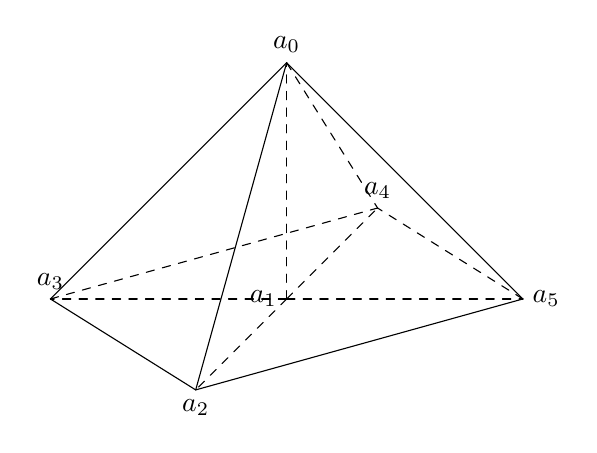
\begin{tikzpicture}[line join = round, line cap = round]
\coordinate [label=left:$a_1$] (A) at (0,0,0);
\coordinate [label=below:$a_2$] (D) at (0,0,3);
\coordinate [label=right:$a_5$] (B) at (3,0,0);
\coordinate [label=above:$a_0$] (C) at (0,3,0);
\coordinate [label=above:$a_3$] (E) at (-3,0,0);
\coordinate [label=above:$a_4$] (F) at (0,0,-3);

\foreach \i in {B,C,D,E,F}
    \draw[dashed] (0,0)--(\i);
\draw[dashed] (B)--(F);
\draw[dashed] (C)--(F);
\draw[dashed] (E)--(F);
\draw[-] (C)--(B);
\draw[-] (C)--(D);
\draw[-] (C)--(E);
\draw[-] (B)--(D);
\draw[-] (D)--(E);
\end{tikzpicture}
\end{figure}
with
\begin{align*}
a_0 &= (-1,-1,1) & a_1 &= (-1,-1,-1) & a_2 &= (1,-1,-1)\\
a_3 &= (-1,-3,-1) & a_4 &= (-3,-1,-1) & a_5 &= (-1,1,-1)
\end{align*}
\begin{align*}
e_0 &= [a_1,a_2] & e_1 &= [a_2,a_0] & e_2 &= [a_0,a_1]\\
e_3 &= [a_0,a_3] & e_4 &= [a_1,a_3] & e_5 &= [a_3,a_2]\\
e_6 &= [a_4,a_5] & e_7 &= [a_0,a_5] & e_8 &= [a_0,a_4]\\
e_9 &= [a_1,a_4] & e_{10} &= [a_5,a_1] & e_{11} &= [a_2,a_5]\\
& & e_{12} &= [a_4,a_3] & &
\end{align*}
Then $M=13,N=1,K=6,J=6,L=5$, so $C$ has $13$ lines and $7$ colons and :
\[
c=\begin{pmatrix}
0 & 0 & -1 & 1 & 0 & 0 & 0 \\
 0 & 1 & 0 & -1 & 0 & 0 & 0 \\
 1 & -1 & 1 & 0 & 0 & 0 & 0 \\
 0 & -1 & 0 & 0 & 1 & 0 & 0 \\
 0 & 0 & -1 & 0 & 1 & 0 & 0 \\
 0 & 0 & 0 & -1 & 1 & 0 & 0 \\
 0 & 0 & 0 & 0 & 0 & -1 & 1 \\
 0 & 1 & 0 & 0 & 0 & 0 & -1 \\
 0 & -1 & 0 & 0 & 0 & 1 & 0 \\
 0 & 0 & 1 & 0 & 0 & -1 & 0 \\
 0 & 0 & 1 & 0 & 0 & 0 & -1 \\
 0 & 0 & 0 & 1 & 0 & 0 & -1 \\
 0 & 0 & 0 & 0 & 1 & -1 & 0 \\
\end{pmatrix}\]

To test this matrix, I created a function which belongs to $\ZZ_h$. For this I used a function $f_{Sh}$ of $\LLL_h$ and set it to be $\varphi_3 - 2\varphi_5$.
I use also a function $\mbf{f}_{Vh}$ in $\NN_h$ and set it to $\mbf{\phi}_2$, which is the only degree of freedom which is not on the boundary.\\
And I computed the function $\mbf{f}=\mbf{f}_{Vh}+\grad f_{Sh}$. This function belongs to $\ZZ_h\subset\NN_h$.\\
\begin{rk}\label{createZh}
  Here is a method to obtain a function in $\ZZ_h$. You use a function in $\LLL_h$ which uses only the basis functions on the boundary, another function in $\NN_h$ which uses only the basis functions in the interior of the domain, and you add the latter and the gradient of the former.\\
  The resultant function belongs to $\ZZ_h$.
\end{rk}
Since the basis of $\ZZ_h$ is $\{\mbf{\phi}_2,\grad\varphi_0,\grad\varphi_1,\grad\varphi_2,\grad\varphi_3,\grad\varphi_4,\grad\varphi_5\}$, we have that 
\begin{align*}
  &&\mbf{f} &= \mbf{\phi}_2 + \grad\varphi_3-2\grad\varphi_5 = (1,0,0,0,1,0,-2) = \alpha\\
  \mbox{but also} &&&\\
  && \mbf{f} &= \mbf{\phi_2} + \mbf{\phi_3} + \mbf{\phi_4} + \mbf{\phi_5} -2 \mbf{\phi_6} +2 \mbf{\phi_7} +2 \mbf{\phi_{10}} +2 \mbf{\phi_{11}} + \mbf{\phi_{12}}\\
  &&&= (0,0,1,1,1,1,-2,2,0,0,2,2,1)
\end{align*}
And we have 
\[
c\ \alpha = \mbf{f}
\]

\subsection{Implementation}
\subsubsection{Details}

For the implementation of this problem, we need several steps :
\begin{itemize}
\item
  create the space $\NN_h$, we can do it using :
  \lstinputlisting[widthgobble=1*2,linerange={Nh,Nh2}]{../../src/basischange.cpp}
\item
  instead of already creating the space $\LLL_h^\Gamma$, we use for now $\LLL_h$ in order to use the same mesh between the two spaces :
  \lstinputlisting[widthgobble=1*2,linerange=P1ch]{../../src/basischange.cpp}
\item
  create the matrix $A$ and $B$ :
  \lstinputlisting[widthgobble=1*2,linerange=forms]{../../src/basischange.cpp}
  The figure \ref{spyA} shows the sparsity pattern of $A$ : 
  \begin{figure}[H]
    \centering
    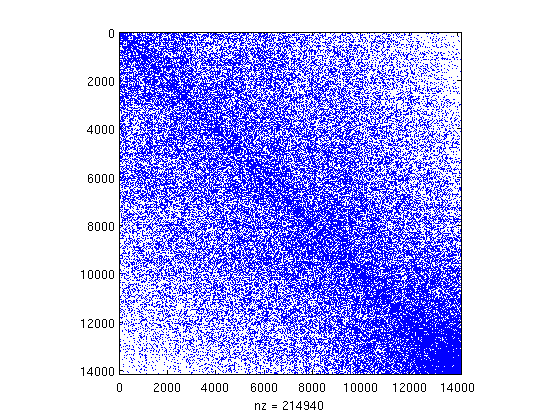
\includegraphics[scale=0.65]{spyA}
    \caption{Sparsity pattern of $A$}
    \label{spyA}
  \end{figure}
\item
  we can now use the function spaces previously defined to retrieve the
  informations on the dofs, if they are on the boundary or if they touch it.\\
  \begin{itemize}
  \item
    We first loop over all the degrees of freedom of $\NN_h$,
    \lstinputlisting[widthgobble=1*2,linerange=loop]{../../src/basischange.cpp}
  \item
    for all these dofs, we retrieve the edge associated and the permutation applied on this edge for the given element, if the permutation is the identity, the sign for the start of the edge is $-1$, else it is $+1$. The sign for the ending point of the edge is the opposite.
    \lstinputlisting[widthgobble=3*2,linerange=perm]{../../src/basischange.cpp}
  \item
    we now search for the dofs of $\LLL_h$ associated with these vertices. For this, we need to find the starting and ending points of the edge, relatively to the elements.\\
    This was the point where we were wrong before.
    \lstinputlisting[widthgobble=3*2,linerange=points]{../../src/basischange.cpp}
    Once we have the find the points, we need to find the corresponding dofs in $\LLL_h$
    \lstinputlisting[widthgobble=4*2,linerange=dofLh]{../../src/basischange.cpp}
  \item
    if the edge is on the boundary,
    \begin{itemize}
    \item
      we set its type,
    \item
      keep the two dofs of $\LLL_h$ corresponding to the vertices in memory,
    \item
      and keep the index of these dofs for later,
    \end{itemize}
  \item
    if the edge is not on the boundary,
    \begin{itemize}
    \item
      we keep the index of the dof for later,
    \item
      and if the two vertices are on the boundary, we set its type such that we
      know that it is {\bf not} on the boundary but it touches it with the two
      vertices, and we also keep the two dofs of $\LLL_h$,
    \item
      if only one vertex is on the boundary, we set its type accordingly, and
      keep the dof concerned,
    \item
      if the edge doesn't touch the boundary, we set its type to remember that.
    \end{itemize}
  \end{itemize}
\item
  we now create two matrices. One of size $M\times M$ for the dofs of $\NN_h$ and one of size $M\times K$ for the dofs of $\LLL_h$.
  \lstinputlisting[linerange=cIntBound]{../../src/basischange.cpp}
\item
  using the informations retrieved on the dofs, we can now fill these two
  matrices :\\
  For each line of the two matrices,
  \begin{itemize}
  \item
    we set the first matrix to be the identity,
  \item
    if the edge touch the boundary with two vertices, we set the columns of
    the second matrix using the indexes of the two dofs corresponding to the
    vertices of the edge,
  \item
    if the edge touch the boundary with only one vertices, the start or the end of the edge, we set only the
    corresponding column,
  \item
    if the edge doesn't touch the boundary, these line stays empty. 
  \end{itemize}
  \lstinputlisting[linerange=fill]{../../src/basischange.cpp}
\item
  we now assemble the two matrices in one matrix $\tilde{C}$ of size $M\times (M+K)$
  \lstinputlisting[widthgobble=1*2,linerange=ctilde]{../../src/basischange.cpp}
  The figure \ref{spyCTilde} shows the sparsity pattern of $\tilde{C}$ : 
  \begin{figure}[H]
    \centering
    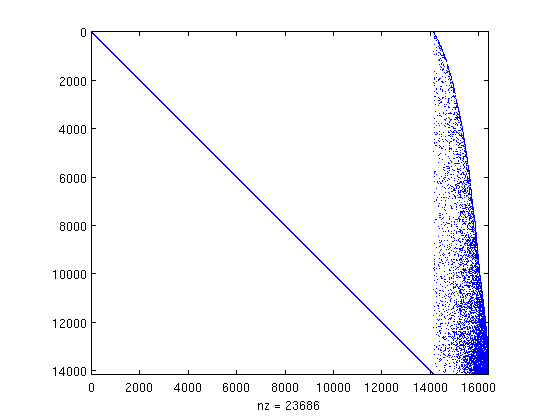
\includegraphics[scale=0.65]{spyCTilde}
    \caption{Sparsity pattern of $\tilde{C}$}
    \label{spyCTilde}
  \end{figure}
\item
  when we retrieved the informations on the dofs, we keep the indexes of the dofs of $\NN_h$ which {\bf are not} on the boundary and the indexes of the dofs of $\LLL_h$ which {\bf are} on the boundary. We only keep the columns of the matrix corresponding to these indexes.
  \lstinputlisting[widthgobble=1*2,linerange=submatrix]{../../src/basischange.cpp}
  The figure \ref{spyC} shows the sparsity pattern of $\tilde{C}$ : 
  \begin{figure}[H]
    \centering
    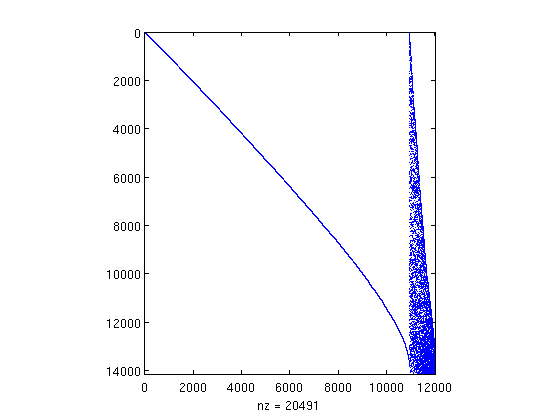
\includegraphics[scale=0.65]{spyC}
    \caption{Sparsity pattern of $C$}
    \label{spyC}
  \end{figure}
\item
  finally, create $\widehat{A}$ and $\widehat{B}$. We use for this the operator \texttt{PtAP} :
  \lstinputlisting[widthgobble=2*2,linerange=ptap]{../../src/basischange.cpp}
  The figure \ref{spyAA} shows the sparsity pattern of $\widehat{A}$ : 
  \begin{figure}[H]
    \centering
    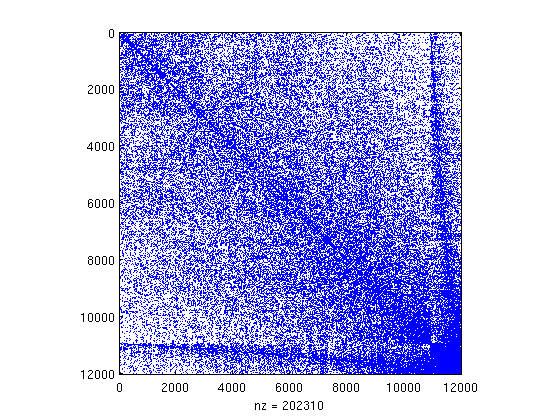
\includegraphics[scale=0.65]{spyAA}
    \caption{Sparsity pattern of $\widehat{A}$}
    \label{spyAA}
  \end{figure}
\item
  We can now resolve the generalized eigen problem with $\widehat{A}$ and $\widehat{B}$.
\item
  Finally, to retrieve the original eigen functions, we need to multiply the eigen functions by $C$.
  \lstinputlisting[widthgobble=2*2,linerange=eigenvec]{../../src/basischange.cpp}
\end{itemize}

\subsubsection{Timing}

The figure \ref{timeC} shows the time take to accomplish the steps for creating the matrix $C$. \texttt{indexes} corresponds to the steps for retrieving the informations on the dofs and the indexes to keep in the matrix. \texttt{fill} corresponds to the steps of creating the two matrices, fill them and assembling them. \texttt{submatrix} corresponds to sorting the vector of indexes, and removing the columns to have $C$. These tests have been conducted on the cylinder.\\

\begin{figure}[H]
  \centering
  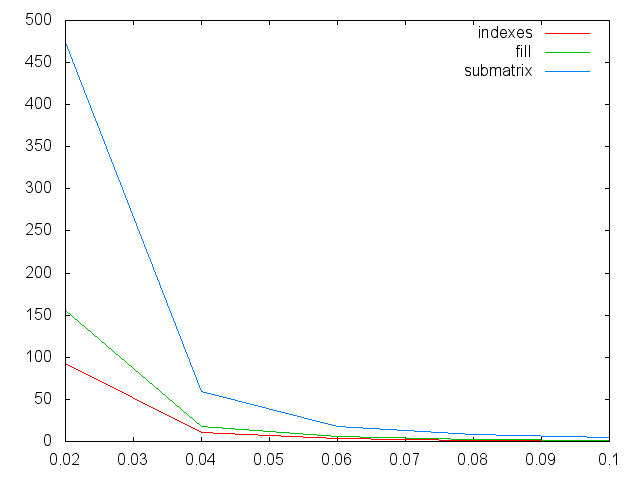
\includegraphics[scale=0.7]{createC}
  \caption{Time to compute C}
  \label{timeC}
\end{figure}

We could think that the time increase really fast but the figure \ref{completeTime} shows the percentage of the total time take for the steps. \texttt{mesh} corresponds to the loading of the mesh, \texttt{space} create $\NN_h$ and $\LLL_h$, and \texttt{forms} create the matrix $A$ and $B$.\\
We see that in fact the percentage of time is constant for each steps.

\begin{figure}[H]
  \centering
  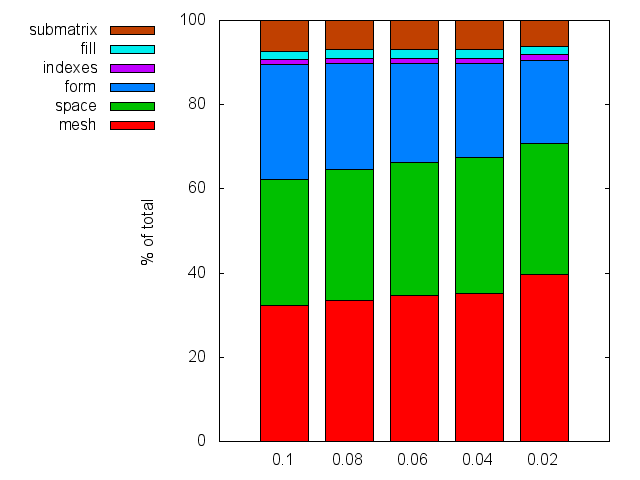
\includegraphics[scale=0.7]{completeChBase}
  \caption{Time to compute the changement of basis}
  \label{completeTime}
\end{figure}

For an idea, we have the following number of dofs depending on the size of the mesh for the cylinder :
\begin{center}
  \begin{tabular}{ c | c | c | c }
    $h$ & \#dof($\NN_h$) & \#dof($\LLL_h$) & \#columns of $C$ \\ \hline
    0.1 & 23\,943 & 3\,908 & 19\,867 \\ \hline
    0.08 & 48\,016 & 7\,593 & 41\,322 \\ \hline
    0.06 & 107\,447 & 16\,414 & 95\,669 \\ \hline
    0.04 & 333\,704 & 49\,202 & 308\,086 \\ \hline
    0.02 & 2\,598\,692 & 367\,288 & 2\,497\,232 \\ \hline
  \end{tabular}
\end{center}

\subsubsection{Results}

I have ran some tests in \texttt{matlab} with the function \texttt{eigs}. 
\paragraph{Sphere}

In the sphere, we know that the first eigen value of the problem \ref{pbstart} is approximately $4.493409$. Since we resolved the problem \ref{pbweak}, our eigen value is squared and with multiplicity 6. So we compute $\widehat{\lambda}_h=(\sum_{i=1}^6\lambda_{i,h})/6$.\\
The table \ref{sphResults} represents the results :
\begin{table}[H]
  \centering
  \begin{tabular}{c|c|ccc|c}
    $\#\NN_h$ & time & $\widehat{\lambda}_h$ & $\lambda$ & $|\widehat{\lambda}_h-\lambda|$ & erc \\
    \hline
    20769 & 2000 & 4.4940 & 4.493409 & 0.000594 & $-$ \\
    44929 & 5000 & 4.4938 & 4.493409 & 0.000359 & 1.6499 \\
    97812 & 34000 & 4.4937 & 4.493409 & 0.000297 & 1.1861 \\
    163559 & 60000 & 4.4936 & 4.493409 & 0.000181 & 1.6112
  \end{tabular}
  \caption{Results in the sphere depending on the number of elements of $\NN_h$}
  \label{sphResults}
\end{table}

The last column is the experimental rate of convergence defined in \cite{Venegas2013} :
\[ erc=-3\frac{\log(|\widehat{\lambda}_h-\lambda|/|\widehat{\lambda}_{h'}-\lambda|)}{\log(\#\NN_h/\#\NN_{h'})} \]
We see that our error is lesser than in their article, but the rate of convergence is better for them than for us.\\

Those are of course prelimenary results and need to be precised with a number of elements way greater. To achieved this, we may need to run in parallel, but we need to review our code in details to be sure it's ok.\\

I created a function to reload the eigen functins from \texttt{Matlab} in \texttt{Feel++}. Using it, I have been able to see the functions in \texttt{Paraview}. The figure \ref{modes} presents the first six modes.
\begin{figure}[H]
	\makebox[\textwidth][c]{
		\subfloat[mode 1]{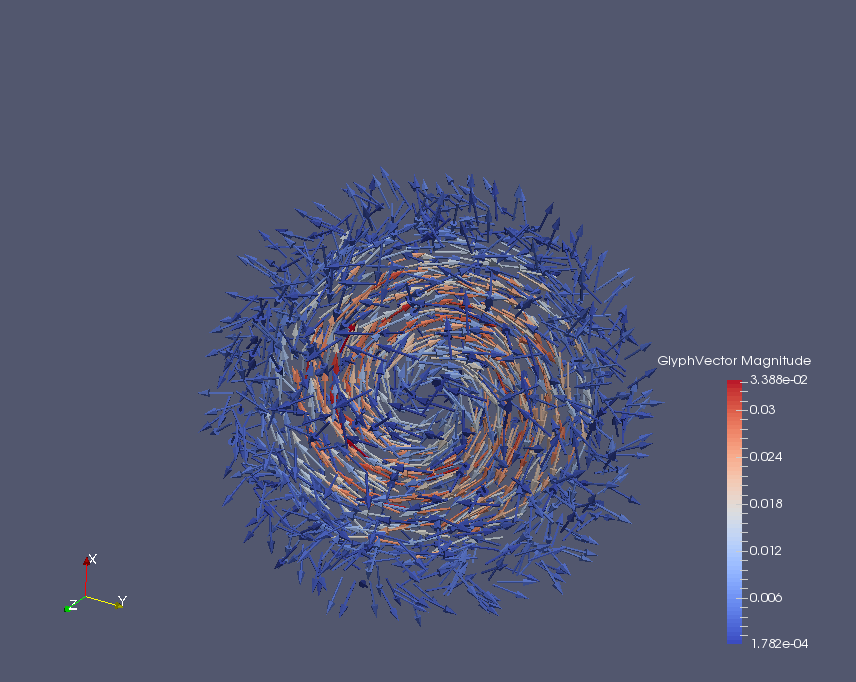
\includegraphics[scale=0.27]{mode1}}\ 
		\subfloat[mode 2]{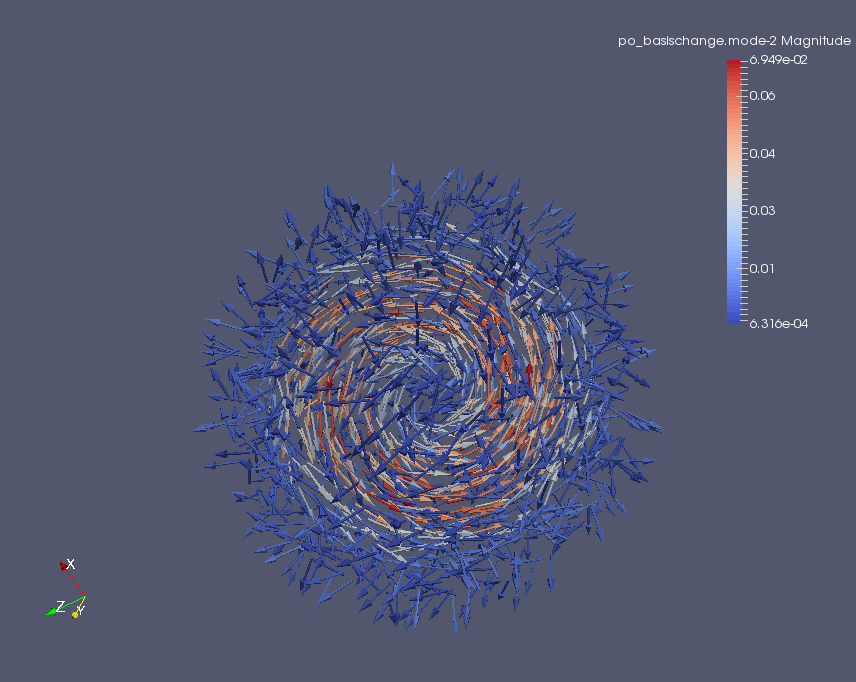
\includegraphics[scale=0.27]{mode2}}
	}\\
	\makebox[\textwidth][c]{
		\subfloat[mode 3]{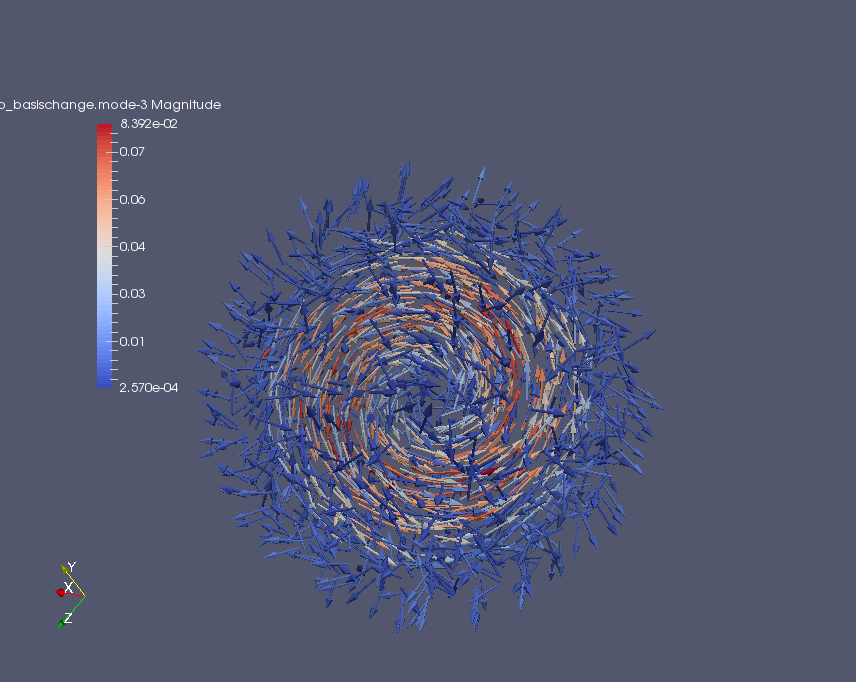
\includegraphics[scale=0.27]{mode3}}\ 
		\subfloat[mode 4]{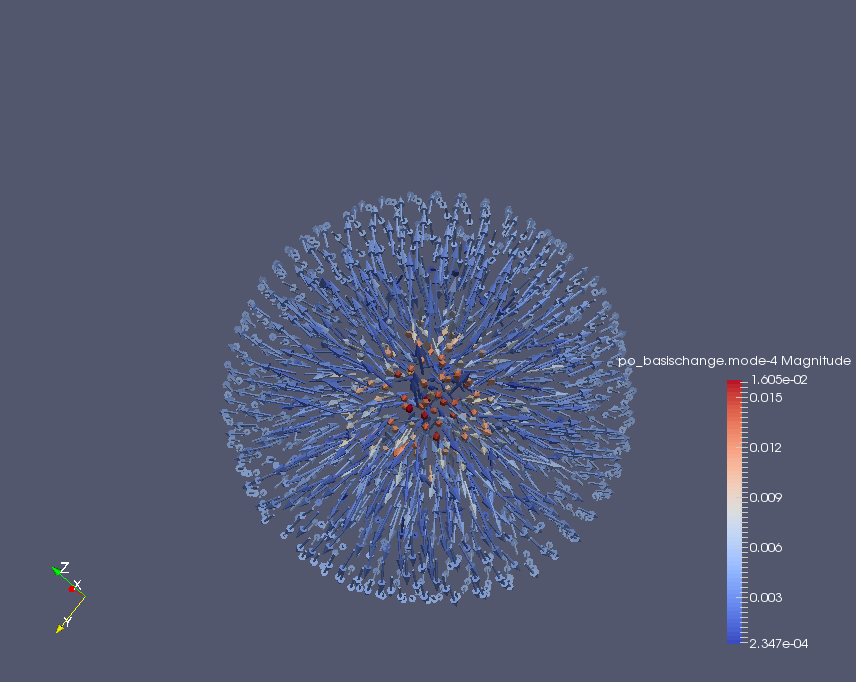
\includegraphics[scale=0.27]{mode4}}
	}\\
	\makebox[\textwidth][c]{
		\subfloat[mode 5]{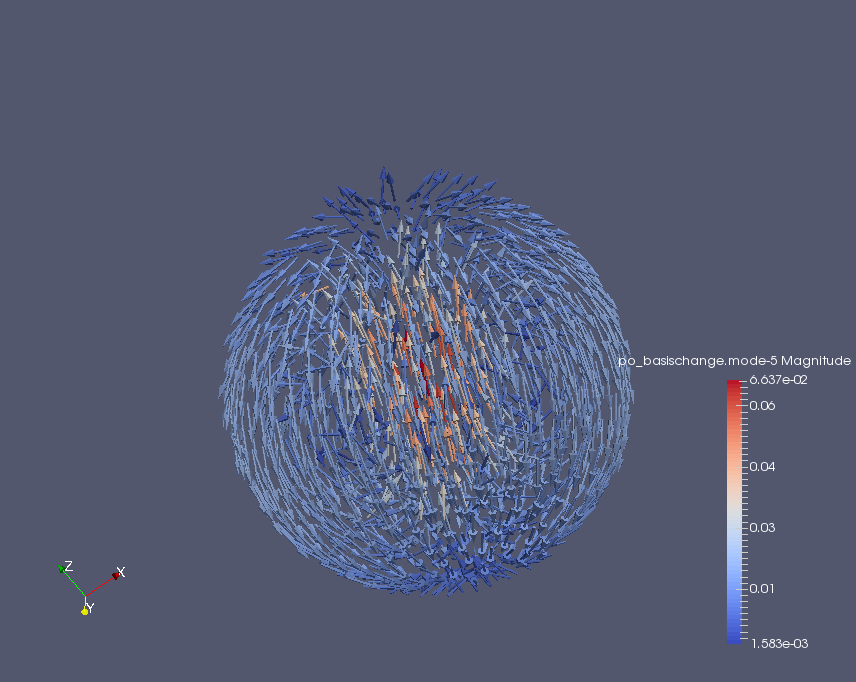
\includegraphics[scale=0.27]{mode5}}\ 
		\subfloat[mode 6]{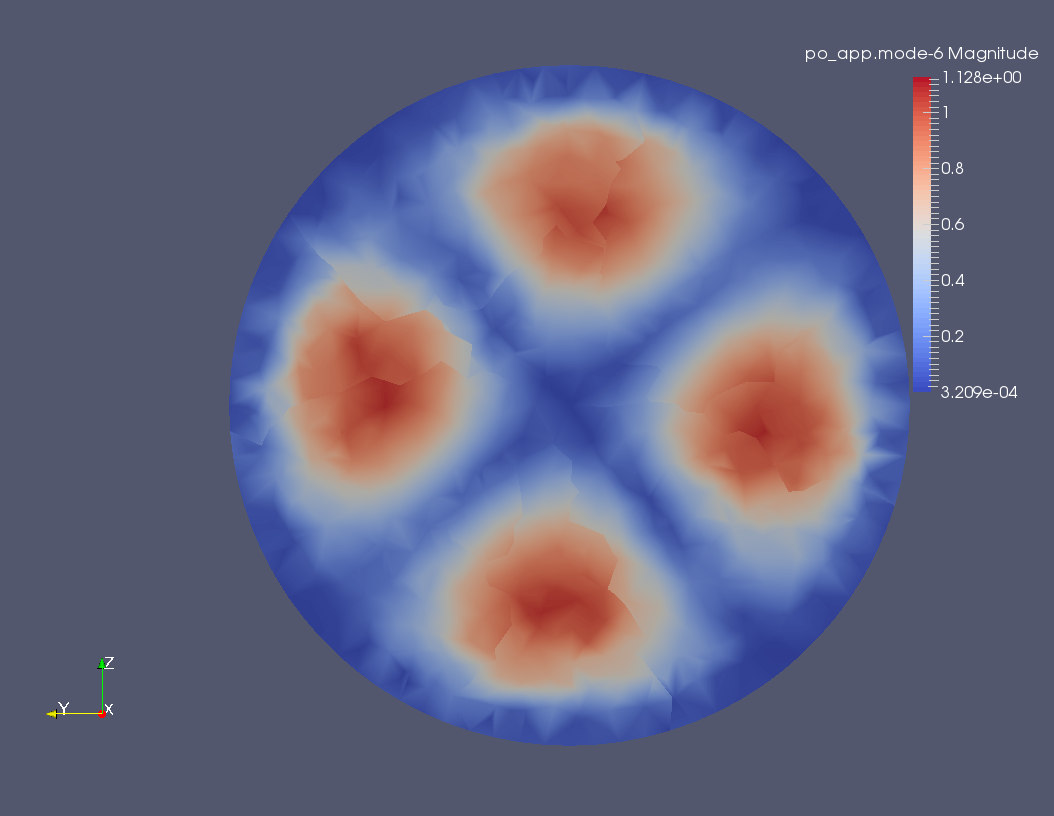
\includegraphics[scale=0.27]{mode6}}
	}
	\caption{Eigen Functions from Matlab}
	\label{modes}
\end{figure}

\paragraph{Rectangular Box}

In the rectangular box, the multiplicity is 2 and we know 3 eigen values : $7.4319, 7.7763, 8.0909$.
\begin{table}[H]
  \centering
  \begin{tabular}{c|cccc|c|c}
    $\#\NN_h$ & 9343 & 35880 & 69501 & 166841 & $\lambda$ & erc \\
    \hline
    time & 330 & 2300 & 7000 & 30544 & $-$ & $-$ \\
    \hline
    $\widehat{\lambda}_{h,1}$ & 7.4215 & 7.4266 & 7.4282 & 7.4298 & 7.4319 & 1.6545 \\
    $\widehat{\lambda}_{h,2}$ & 7.7614 & 7.7702 & 7.7725 & 7.7744 & 7.7763 & 2.1019 \\
    $\widehat{\lambda}_{h,3}$ & 8.0732 & 8.0825 & 8.0848 & 8.0869 & 8.0909 & 1.5158
  \end{tabular}
  \caption{Results in the rectangular box depending on the number of elements of $\NN_h$}
  \label{RBResults}
\end{table}
We can notice in table \ref{RBResults} that the time of computation for the greater number of elements is way smaller than in the sphere. I need to check this with a larger set of element's size.

\paragraph{Back in \texttt{Feel++}}

Using the following configuration :
\begin{description}
\item[solver] krylovschur
\item[problem] ghep
\item[transform] shift\_invert
\item[interval] 19,21
\end{description}
I find the 6 first eigenvalue in the sphere.\\
The \texttt{interval}  option is \texttt{eps\_interval}, which retrieve all the eigenvalues in a given interval. This interval can be open in one end, so we could use $[a, \infty)$ with $a$ very small but positive.\\
There is some limitations with this option as exposed in the \href{http://slepc.upv.es/documentation/slepc.pdf}{documentation of SLEPc} \S 3.4.5. We have to use KrylovSchur as solver and shift and invert as transform.\\
Furthermore, direct linear solvers are required. This linear solver must provide the matrix inertia and must use a symmetric factorization (\texttt{cholesky}).\\
To use it in parallel, we have to use MUMPS.\\
So the command looks like :\\ \texttt{./feelpp\_po\_basischange --solvereigen.solver krylovschur -eps\_interval 19,30 -st\_ksp\_type preonly -st\_pc\_type cholesky -st\_pc\_factor\_mat\_solver\_package mumps -mat\_mumps\_icntl\_13 1}\\

\begin{figure}[H]
  \makebox[\textwidth][c]{
    \subfloat[Sphere]{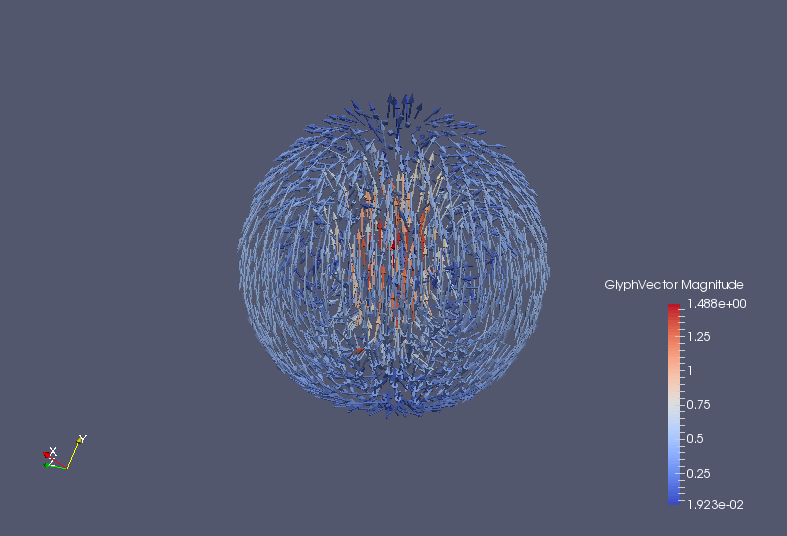
\includegraphics[scale=0.27]{sphMode0}}\ 
    \subfloat[Rectangular Box]{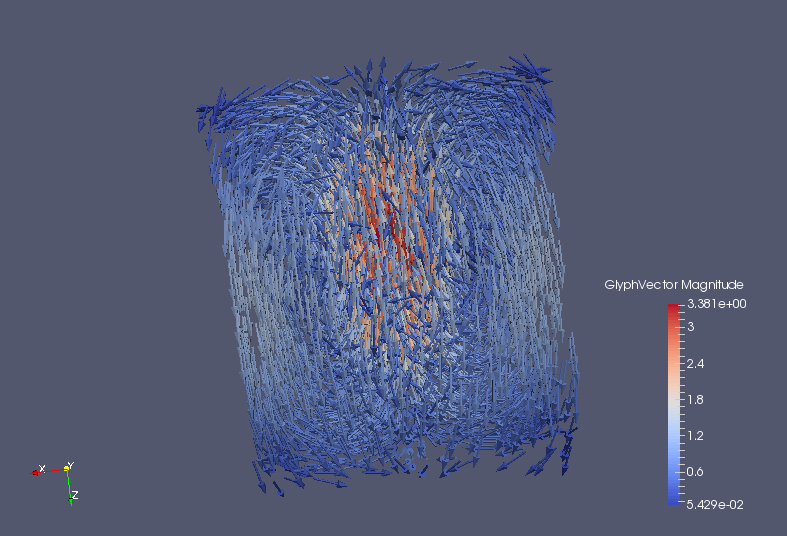
\includegraphics[scale=0.27]{rbMode0}}
  }
  \caption{Eigen Functions from Feel++}
  \label{feelModes}
\end{figure}

To understand the link between those functions and the eigen functions of the curl operator, I'll quote the article \cite{Venegas2013} :
\begin{italicquotes}
  According to the theoretical results, the invariant subspace spanned by the six eigenfunctions of Problem \ref{pbdiscr} corresponding to $\lambda_{h,1},\dots,\lambda_{h,6}$ yields an approximation of the eigenspace of $\lambda^2$ in Problem \ref{pbweak}. However, the latter is the direct sum of two three-dimensional eigenspaces of Problem \ref{pbstart}, those corresponding to $\lambda$ and $-\lambda$. Therefore, the eigenfunctions of Problem \ref{pbdiscr} are not in general eigenfunctions of Problem \ref{pbstart} (and hence Beltrami fields), but a linear combination of eigenfunctions corresponding to both eigenvalues, $\lambda$ and $-\lambda$.
\end{italicquotes}

And indeed, we do not have that $\curl\mbf{u}_i-\lambda_i\mbf{u}_i = 0$.\\
For the first eigenvalue, we have the following results :
\begin{table}[H]
  \centering
  \begin{tabular}{r|c|c}
    h & 0.15 & 0.075 \\
    \hline
    $\widehat{\lambda}_h$ & 4.49481924 & 4.49377347\\
    $|\widehat{\lambda}_h-\lambda|$ & 0.00141024 & 0.00036447 \\
    erc & $-$ & \\
    \hline
    $||\div\mbf{u}||_2$ & 2.88311e-14 & 6.60701e-14 \\
    $||\mbf{u}\cdot\mbf{n}||_2$ & 0.216208 & 0.112487 \\
    $||\curl\mbf{u}\cdot\mbf{n}||_2$ & 5.11927e-15 & 9.48309e-15 \\
    $||\curl\mbf{u}-\lambda\mbf{u}||_2$ & 6.5155 & 6.38584
  \end{tabular}
  \caption{Results in the sphere}
\end{table}

\begin{table}[H]
  \centering
  \begin{tabular}{c|cc|c}
    h & 0.075 & 0.05 & $\lambda$ \\
    \hline
    $\widehat{\lambda}_{h,1}$ & 7.42151 & 7.42658 & 7.4319 \\
    $\widehat{\lambda}_{h,2}$ & 7.76569 & 7.77023 & 7.7763 \\
    $\widehat{\lambda}_{h,3}$ & 8.07633 &  8.08247 & 8.0909    
  \end{tabular}
  \caption{Results in the rectangular box}
\end{table}

We can see that the divergence and the normal component of the curl are zero, but the normal component of the function is not exactly zero, but tends to dicrease as $h$ tends to 0.\\
The important thing is that the eigenspaces are equivalents.\\



%%% Local Variables:
%%% TeX-master: "../peps.tex"
%%% eval: (flyspell-mode 1)
%%% ispell-local-dictionary: "english"
%%% End:
